\documentclass[twocolumn,linenumbers]{aastex63}

\usepackage[utf8]{inputenc}
\usepackage{natbib}
\usepackage{graphicx}
\usepackage{amsmath}
\usepackage{booktabs}
\usepackage{longtable}
\usepackage{xspace}
\usepackage{hyperref}
\usepackage[T1]{fontenc}
\usepackage{comment}
\usepackage{xcolor}
\usepackage{enumitem}
\usepackage{multirow}
\usepackage{rotating}

% Operator names, carried over from the AstroQ methods paper so the notation
% matches between the two.
\def\over{\mathrm{over}}
\def\read{\mathrm{read}}
\def\slew{\mathrm{slew}}
\def\Overhead{\mathrm{Overhead}}
\def\inter{\mathrm{inter}}
\def\intra{\mathrm{intra}}
\def\slot{\mathrm{slot}}

\def\multivisit{\mathrm{multi-visit}}
\def\singlevisit{\mathrm{single-visit}}

\def\Acal{\mathcal{A}}
\def\Dcal{\mathcal{D}}
\def\Ical{\mathcal{I}}
\def\Jcal{\mathcal{J}}
\def\Pcal{\mathcal{P}}
\def\Rcal{\mathcal{R}}
\def\Scal{\mathcal{S}}
\def\Tcal{\mathcal{T}}

\newcommand{\red}[1]{\textcolor{red}{#1}}
\newcommand{\blue}[1]{\textcolor{blue}{#1}}
\newcommand{\AstroQ}{\textit{AstroQ}\xspace}
\newcommand{\tauslot}{\ensuremath{\tau_{\rm slot}}\xspace}
\newcommand{\taurm}[1]{\ensuremath{\tau_{\rm #1}}\xspace}
\newcommand{\isr}[2]{\ensuremath{#1_{\rm #2}}\xspace}
\newcommand\round[1]{\left[#1\right]}

% Program-balance notation introduced by this paper.
\newcommand{\Fp}{\ensuremath{F_p}\xspace}
\newcommand{\maff}{\ensuremath{F^{\rm max}_p}\xspace}
\newcommand{\fsf}{\ensuremath{\sigma_p}\xspace}
\newcommand{\fsfmax}{\ensuremath{\sigma_{\rm max}}\xspace}
\newcommand{\minfill}{\ensuremath{F^{\rm min}_p}\xspace}
\newcommand{\maxfill}{\ensuremath{F^{\rm cap}_p}\xspace}
\newcommand{\Zstar}{\ensuremath{Z^{\star}}\xspace}

% params.tex is generated by tools/make_params.py from the artifacts in data/.
% Every measured number in the prose must be written as \param{key}; an
% unresolved key renders as a red XX rather than disappearing silently.
% GENERATED by tools/make_params.py -- do not edit by hand.
% Regenerate with: make params
\usepackage{xparse}
\usepackage{xcolor}
\usepackage{etoolbox}
\ExplSyntaxOn
\NewDocumentCommand{\param}{m}{
\str_case:nnF {#1} {
{base-alloc-slots}{4937}%
{base-awarded}{164.5}%
{base-balance-gap}{62.0}%
{base-balance-seconds}{60}%
{base-capacity}{164.55}%
{base-fill-balance-stage}{93}%
{base-fill-shortfall-stage}{93}%
{base-idle}{8.78}%
{base-nblocks}{29}%
{base-nprograms}{9}%
{base-requested}{198.1}%
{base-scheduled}{155.77}%
{base-shortfall-cap}{1101.1}%
{base-shortfall-drift}{+0.0}%
{base-shortfall-final}{1001}%
{base-shortfall-gap}{0.0}%
{base-shortfall-objective}{1001}%
{base-shortfall-seconds}{326}%
{base-subscription}{120}%
{base-u258-award}{36.10}%
{base-u258-donated-hours}{24.77}%
{base-u258-donated-nights}{4}%
{base-u258-maff}{0.71}%
{base-u258-proj}{25.70}%
{base-worst-fsf-after}{0.005}%
{base-worst-fsf-after-prog}{C275}%
{base-worst-fsf-before}{0.005}%
{base-worst-fsf-before-prog}{C275}%
{drop2-alloc-slots}{4573}%
{drop2-awarded}{152.4}%
{drop2-balance-gap}{1.2}%
{drop2-balance-seconds}{600}%
{drop2-capacity}{152.42}%
{drop2-dropped-hours}{12.13}%
{drop2-dropped-nights}{2}%
{drop2-fill-balance-stage}{100}%
{drop2-fill-shortfall-stage}{99}%
{drop2-idle}{0.62}%
{drop2-nblocks}{27}%
{drop2-nprograms}{9}%
{drop2-requested}{198.1}%
{drop2-scheduled}{151.80}%
{drop2-shortfall-cap}{1181.4}%
{drop2-shortfall-drift}{-1.0}%
{drop2-shortfall-final}{1063}%
{drop2-shortfall-gap}{2.3}%
{drop2-shortfall-objective}{1074}%
{drop2-shortfall-seconds}{300}%
{drop2-subscription}{130}%
{drop2-u258-award}{23.97}%
{drop2-u258-maff}{1.00}%
{drop2-u258-proj}{23.60}%
{drop2-worst-fsf-after}{0.005}%
{drop2-worst-fsf-after-prog}{H402}%
{drop2-worst-fsf-before}{0.019}%
{drop2-worst-fsf-before-prog}{U252}%
{pair-awarded}{164.5}%
{pair-balance-gap-max}{62}%
{pair-balance-loose}{8}%
{pair-balance-timelimit}{300}%
{pair-blip-date}{2026-09-18}%
{pair-c275-dip-bal}{0.87}%
{pair-c275-dip-nobal}{0.81}%
{pair-frozen-final-bal}{0.130}%
{pair-frozen-final-nobal}{0.140}%
{pair-frozen-peak-bal}{0.130}%
{pair-frozen-peak-nobal}{0.190}%
{pair-fsf-final-bal}{0.030}%
{pair-fsf-final-nobal}{0.030}%
{pair-fsf-mean-bal}{0.017}%
{pair-fsf-mean-nobal}{0.030}%
{pair-fsf-peak-bal}{0.050}%
{pair-fsf-peak-nobal}{0.140}%
{pair-hours-bal}{144.5}%
{pair-hours-nobal}{144.6}%
{pair-lost}{5}%
{pair-lost-frac}{17}%
{pair-nights}{29}%
{pair-nprograms}{9}%
{pair-protected}{4}%
{pair-seed}{1}%
{pair-shortfall-converged-bal}{29}%
{pair-shortfall-converged-nobal}{29}%
{pair-shortfall-gap-max-bal}{0.3}%
{pair-shortfall-gap-max-nobal}{0.2}%
{pair-spared-mean-bal}{0.012}%
{pair-spared-nobal}{6}%
{pair-split-date}{2026-10-18}%
{pair-squeezed}{5}%
{pair-squeezed-hi}{0.96}%
{pair-squeezed-lo}{0.95}%
{pair-u258-dip-bal}{0.62}%
{pair-u258-dip-nobal}{0.58}%
{pair-weather-p}{25}%
{pipeline-hold-alpha}{0.0}%
{pipeline-maxfill-late}{1.25}%
{pipeline-mipgap}{0.005}%
{pipeline-slack}{1.1}%
{pipeline-slack-pct}{10}%
{pipeline-slot-minutes}{2}%
{pipeline-stages}{5}%
{wx-balance-timelimit}{600}%
{wx-hires-balance-gap-p90}{57.8}%
{wx-hires-fill-realized-mean}{0.828}%
{wx-hires-fill-spread}{1.285}%
{wx-hires-fsf-start-max}{0.141}%
{wx-hires-nights}{29}%
{wx-hires-replans}{7}%
{wx-hires-seed}{24}%
{wx-hires-shortfall-gap-p90}{0.4}%
{wx-hires-weather-frac}{21}%
{wx-shortfall-norel}{300}%
{wx-shortfall-timelimit}{900}%
{wx-toy-balance-gap-p90-max}{0.8}%
{wx-toy-fill-realized-mean}{0.366}%
{wx-toy-fill-spread-max}{0.136}%
{wx-toy-fill-spread-mean}{0.087}%
{wx-toy-fsf-start-max}{0.718}%
{wx-toy-nights}{49}%
{wx-toy-replans-mean}{15}%
{wx-toy-seeds}{3}%
{wx-toy-weather-frac-mean}{29}%
{wx-weather-p}{0.25}%
}{{\color{red}XX}}  % fallback
}
\ExplSyntaxOff


\begin{document}

\title{Operating a Cadence-Scheduled Queue: Lessons from HIRES 2026B}

\author[0000-0003-0967-2893]{Erik A. Petigura}
\affiliation{Department of Physics \& Astronomy, University of California Los Angeles, Los Angeles, CA 90095, USA}

\begin{abstract}
\red{Placeholder.} We report on the first semester of operating the
California Planet Search HIRES queue under \AstroQ, the automated cadence
scheduler of \citet{Lubin2025}. \red{Findings to be drafted; see notes/ for the
running record of results and their provenance.}
\end{abstract}

\keywords{scheduling optimization, radial velocities}

\section{Introduction}
\label{sec:intro}

\red{To be drafted.} Motivation: what changes when an automated cadence
scheduler moves from simulation onto a real oversubscribed queue.

\section{The HIRES 2026B Queue}
\label{sec:queue}

\red{To be drafted.} Programs, awards, request volume, and the allocation as
delivered by Keck. Table~\ref{tab:semester} summarizes the queue as planned on
the first night of the semester, and Figure~\ref{fig:football} shows where its
targets lie.

\begin{figure*}
  \centering
  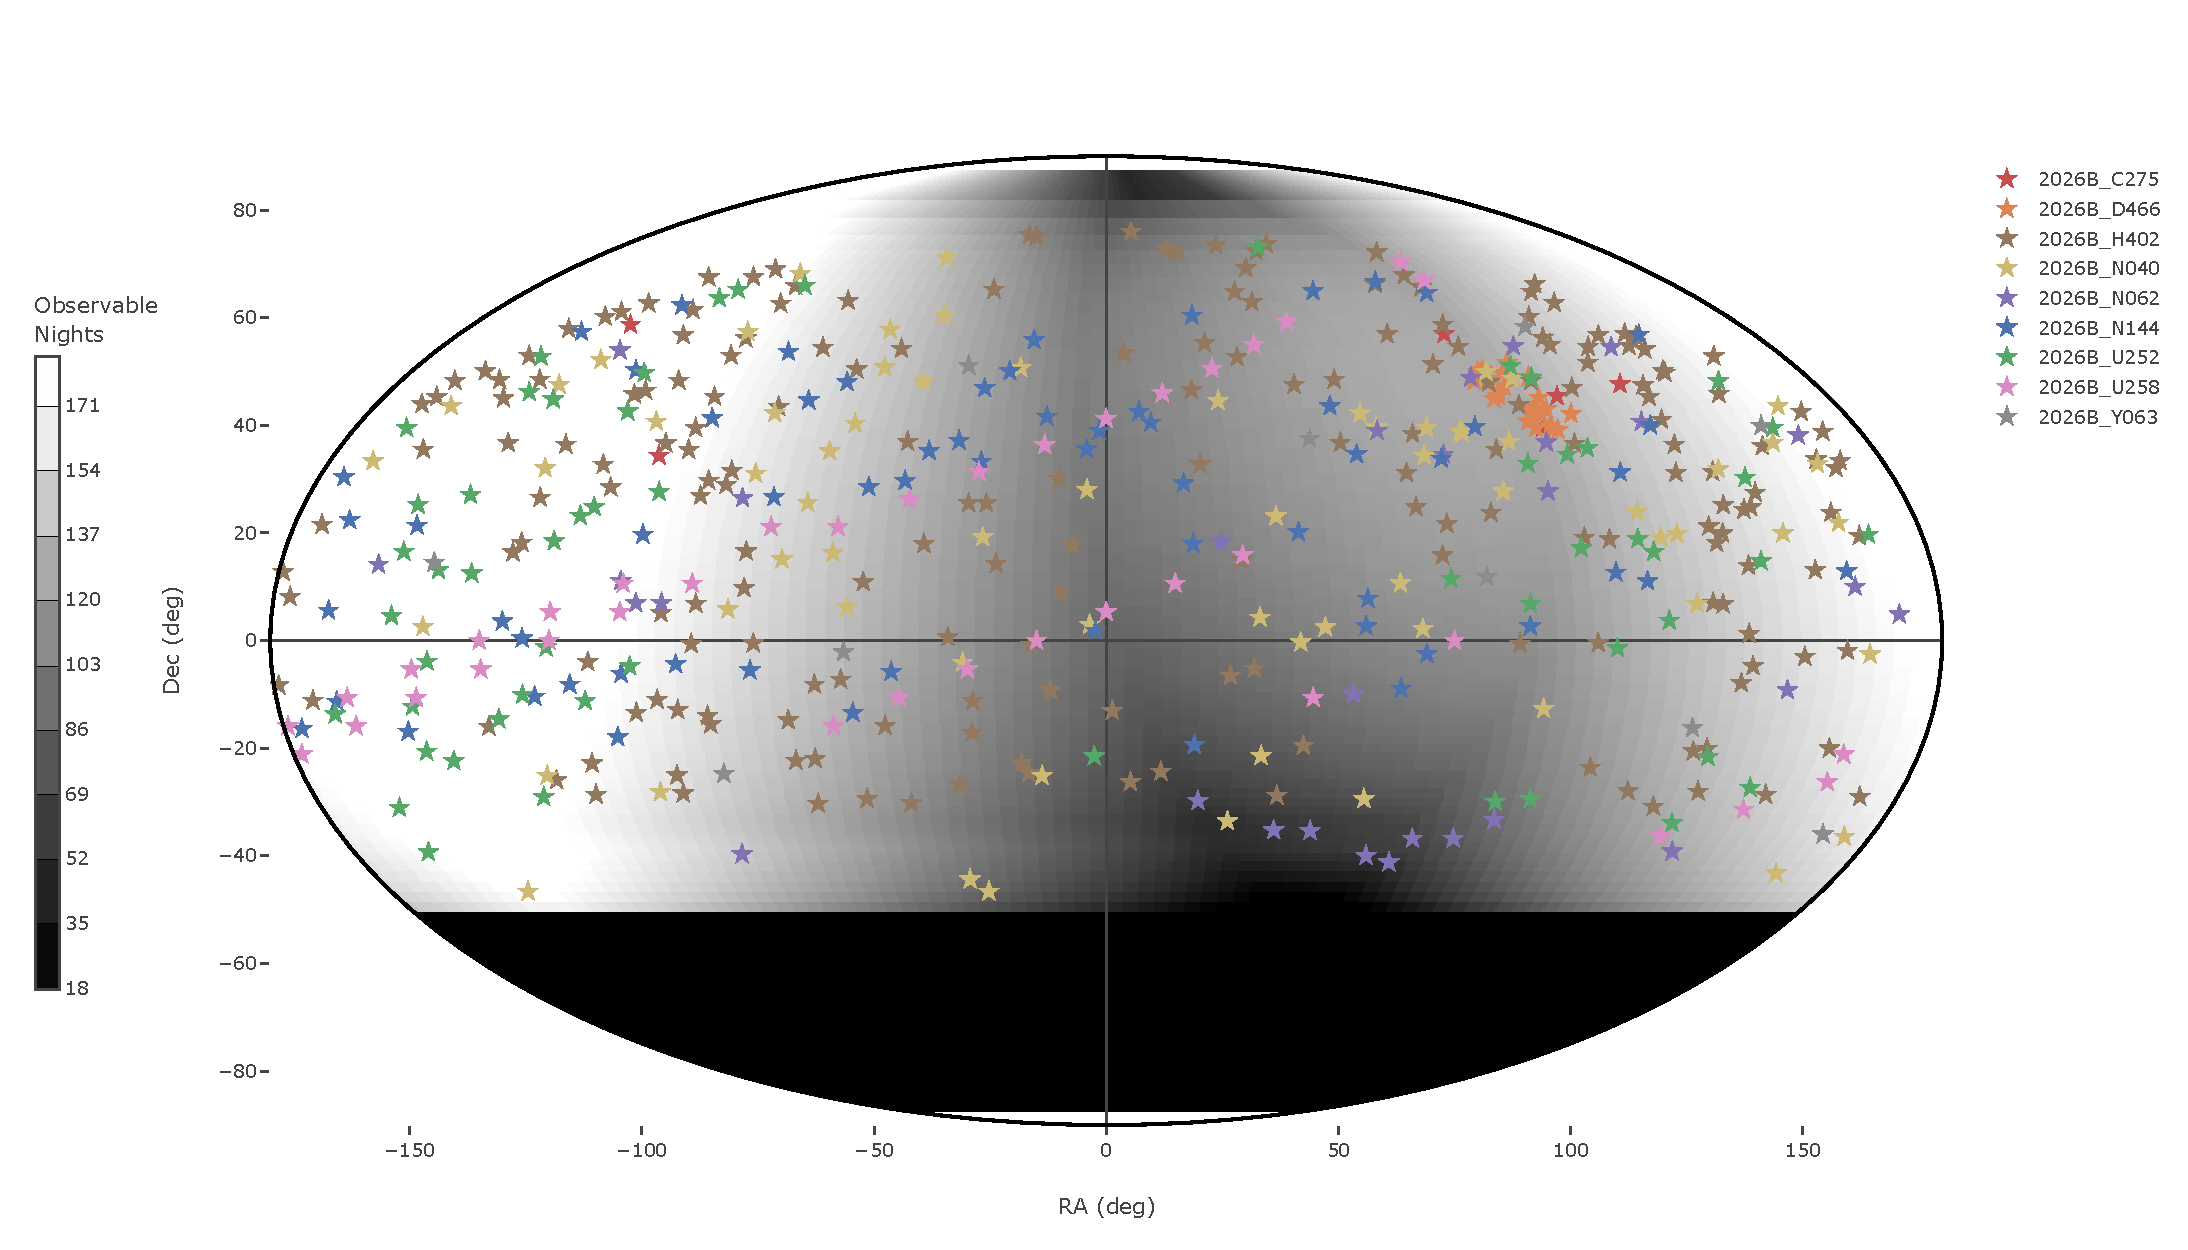
\includegraphics[width=\textwidth]{plots/football.pdf}
  \caption{Requests in the 2026B HIRES queue, colored by program, over a
  grayscale map of the number of nights in the semester on which each part of
  the sky is observable from Maunakea. Programs are broadly dispersed in right
  ascension, so most compete for the same well-placed sky rather than for
  particular nights. \red{Caption to be finalized.}}
  \label{fig:football}
\end{figure*}

% GENERATED by tools/make_tables.py -- do not edit by hand.
\begin{deluxetable}{lr}
\tablecaption{Semester-level statistics for the 2026B HIRES queue, as planned on the first night\label{tab:semester}}
\tablehead{\colhead{Quantity} & \colhead{Value}}
\startdata
Requests submitted & 534 \\
Requests active & 529 \\
Requests schedulable & 512 \\
Time requested & 198.0 hr \\
Time allocated & 164.6 hr \\
Time scheduled & 155.8 hr \\
Semester fill factor & 95\% \\
Time allocated, first night & 9.3 hr \\
Time scheduled, first night & 9.3 hr \\
Fill factor, first night & 100\%
\enddata
\tablecomments{Time is reported in hours, converted from the \param{pipeline-slot-minutes}~min scheduling slot. Requested time counts every visit a PI asked for and so exceeds the allocation; see \S\ref{sec:balance:nocompete}. The fill factor is the fraction of allocated time occupied by a scheduled visit.}
\end{deluxetable}


\section{The Five-Stage Optimization}
\label{sec:stages}

\subsection{From one objective to five}
\label{sec:stages:motivation}

\citet{Lubin2025} pose semester scheduling as a single mixed-integer program.
One objective is minimized,

\begin{equation}
  Z = \sum_{r \in \Rcal} \Theta_r \isr{t}{visit,r},
  \label{eq:obj-shortfall}
\end{equation}

\noindent where $\Theta_r$ is the shortfall of request $r$: the number of
requested visits, net of those already executed, that the schedule fails to
deliver. Because $\Theta_r$ is floored at zero, the objective does not reward
visits beyond \isr{n}{inter,r}. The model is solved once and the resulting
$Y_{r,d,s}$ is the schedule.

A single objective is sufficient to answer a single question, namely how many
of the requested visits can be delivered. Operating a real queue raises three
further questions that Equation~\ref{eq:obj-shortfall} is silent on. Among the
many schedules that deliver equally many visits, which one distributes the
delivered time most evenly across programs? Within a program, which targets
should be favored when not all of them fit? And what should be done with
allocated time that the shortfall objective has no incentive to use, since
extra visits earn nothing?

We answer these by solving \param{pipeline-stages} problems in sequence rather
than one. Each stage installs a new objective on the same model, retaining the
constraints accumulated by its predecessors, so that later stages break ties
left by earlier ones without undoing them. This is a lexicographic, or
$\varepsilon$-constraint, treatment of a multi-objective problem: earlier
objectives take strict precedence, but are held only to within a stated
tolerance so that later objectives have room to act.

\subsection{Program fill factor}
\label{sec:stages:fill}

Equation~\ref{eq:obj-shortfall} contains no notion of a program. Requests carry
cadence requirements, and a program is merely the set of requests that share a
PI. To reason about balance we introduce the program as a modeled entity.

Let $p \in \Pcal$ index programs and let $\Rcal_p \subset \Rcal$ be the requests
belonging to program $p$. Each program is awarded $A_p$ slots of telescope time
and has already executed $\isr{A}{past,p}$ slots. We define the fill factor \Fp
as a continuous decision variable linked to the schedule by

\begin{equation}
  \Fp A_p = \isr{A}{past,p} + \sum_{r \in \Rcal_p} \ \sum_{(d,s) \in \mathcal{A}_r}
  \isr{t}{visit,r} \, Y_{r,d,s} .
  \label{eq:fill-link}
\end{equation}

\noindent \Fp is therefore the projected time a program will receive over the
whole semester, past and future, as a fraction of its award. A program that
exactly consumes its award has $\Fp = 1$. Bounds

\begin{equation}
  \minfill \le \Fp \le \maxfill
  \label{eq:fill-bounds}
\end{equation}

\noindent are reset at the start of each stage, and it is by moving \maxfill
between stages that the pipeline separates the question of who gets their
award from the question of who gets the leftovers.

\subsection{Stage 1: shortfall}
\label{sec:stages:shortfall}

The first stage reproduces \citet{Lubin2025}: minimize
Equation~\ref{eq:obj-shortfall} subject to the accessibility, cadence, and
non-overlap constraints of that work. The one addition is the ceiling
$\maxfill = 1$, which forbids any program from consuming more than its award
while the delivery question is being settled. Without it a program with a dense
request list could absorb time that a thinner program is entitled to, and no
later stage could recover it.

We record the optimum \Zstar and the resulting fill factors $\Fp^{(1)}$.

\subsection{Stage 2: balance}
\label{sec:stages:balance}

Programs differ in how much of their award they could ever use. A program whose
targets are visible all semester can reach $\Fp = 1$; a program whose nights
fall outside its observing season cannot, no matter how favorably it is
treated. We therefore measure each program not against unity but against the
best it could do alone. The maximum feasible fill \maff is the fill program $p$
attains when scheduled with the telescope to itself, computed by a separate
solve of Equation~\ref{eq:obj-shortfall} restricted to $\Rcal_p$. The fill
shortfall is

\begin{equation}
  \fsf = \maff - \Fp ,
  \label{eq:fsf}
\end{equation}

\noindent and the stage minimizes the worst of them,

\begin{equation}
  \fsfmax = \max_{p \in \Pcal} \ \fsf ,
  \label{eq:fsfmax}
\end{equation}

\noindent implemented as a single continuous variable with $\fsfmax \ge \fsf$
for every $p$. Minimizing a maximum in this way is the standard linear
reformulation and keeps the model an MILP.

Balance must not be bought by delivering fewer visits, so
Equation~\ref{eq:obj-shortfall} is retained as a constraint,

\begin{equation}
  \sum_{r \in \Rcal} \Theta_r \isr{t}{visit,r} \le \alpha \Zstar ,
  \label{eq:shortfall-cap}
\end{equation}

\noindent with $\alpha = \param{pipeline-slack}$. The stage may thus give up at
most \param{pipeline-slack-pct}\% of the delivered visit-time in exchange for a
more even distribution of it. The bounds of
Equation~\ref{eq:fill-bounds} are reset to $\maxfill = 1$ and the operator
floors, deliberately \emph{not} to $\Fp^{(1)}$: on a fully subscribed telescope
raising the worst program requires lowering some other, so freezing every
program at its stage-1 fill would make the stage a no-op.

Measuring against \maff rather than against unity is what distinguishes this
from raising a common floor on \Fp. A floor is held hostage by the least
fillable program in the queue, which caps how high the floor can rise no matter
how well the remaining programs are doing. Equation~\ref{eq:fsf} excuses a
program for time it could never have used and holds it responsible only for
time it lost to its neighbors.

\subsection{Stage 3: prioritize}
\label{sec:stages:prioritize}

Stages 1 and 2 treat all requests within a program as interchangeable. PIs do
not. Each request carries a weight $w_r$, with smaller values denoting higher
priority, and this stage maximizes

\begin{equation}
  \sum_{(r,d,s) \in \Acal} \frac{1}{w_r} \, Y_{r,d,s}
  \label{eq:obj-prioritize}
\end{equation}

\noindent so that, among schedules of equal quality by the preceding measures,
the one favoring each PI's preferred targets is selected. The balance result is
locked in here rather than in stage 2, by setting
$\minfill = (1 - \alpha_{\rm hold}) \Fp^{(2)}$ with
$\alpha_{\rm hold} = \param{pipeline-hold-alpha}$, which pins each program at
the fill it was assigned.

This stage also raises the ceiling to $\maxfill = \param{pipeline-maxfill-late}$.
Once the division of the award is settled, a program may overrun its award to
take up time that would otherwise go unused. The consequences of this ordering
are the subject of \S\ref{sec:balance}.

\subsection{Stage 4: fill-empty}
\label{sec:stages:fillempty}

Because $\Theta_r$ is floored at zero, no earlier objective rewards a visit
beyond \isr{n}{inter,r}, and allocated time for which every request is already
satisfied is simply left empty. On a queue where some programs cannot use their
nights, that idle time is substantial. This stage recovers it by minimizing

\begin{equation}
  \sum_{(d,s) \in \Tcal_{\rm alloc}} 1
  \ - \sum_{(r,d,s) \in \Acal} \isr{t}{visit,r} \, Y_{r,d,s},
  \label{eq:obj-fillempty}
\end{equation}

\noindent the allocated slot-time that no visit occupies. To ensure that
packing the schedule does not displace a scheduled visit, the per-request
shortfalls are frozen individually,

\begin{equation}
  \Theta_r \le \Theta_r^{(3)} \qquad \forall r \in \Rcal .
  \label{eq:theta-freeze}
\end{equation}

\noindent This is stronger than Equation~\ref{eq:shortfall-cap}, which bounds
only the weighted sum and would permit one request to be dropped so that
another could be added.

\subsection{Stage 5: fill-current-day}
\label{sec:stages:fillcurrent}

The semester plan is re-solved every afternoon, and its operational product is
not the semester but the script for the coming night. All nights are equivalent
to the preceding objectives, so the solver has no reason to prefer a schedule
that packs tonight over one that packs an arbitrary night in November. The
final stage removes that indifference by maximizing the slot-time used on the
upcoming night $d_0$,

\begin{equation}
  \sum_{r \in \Rcal} \ \sum_{s \in \Scal} \isr{t}{visit,r} \, Y_{r,d_0,s},
  \label{eq:obj-fillcurrent}
\end{equation}

\noindent again subject to Equation~\ref{eq:shortfall-cap}. Visits pulled
forward into tonight are ones the semester plan intended to make anyway, so the
cost is borne by later nights, which will be re-planned tomorrow.

\subsection{Summary}
\label{sec:stages:summary}

Table~\ref{tab:stages} collects the five stages. Constraints are cumulative
down the table; the final column gives the interval to which \Fp is bounded at
the start of each stage, where \minfill is the operator-supplied floor from
\texttt{programs.csv}.

\begin{deluxetable*}{llll}
\tablecaption{The \param{pipeline-stages}-stage semester optimization\label{tab:stages}}
\tablehead{
  \colhead{Stage} & \colhead{Objective} & \colhead{Constraint added} &
  \colhead{Bounds on \Fp}
}
\startdata
1. shortfall & min $\sum_r \Theta_r \isr{t}{visit,r}$ & --- & $[\minfill, 1]$ \\
2. balance & min \fsfmax & $\sum_r \Theta_r \isr{t}{visit,r} \le \alpha \Zstar$ & $[\minfill, 1]$ \\
3. prioritize & max $\sum_{r,d,s} Y_{r,d,s} / w_r$ & --- & $[F^{(2)}_p, \param{pipeline-maxfill-late}]$ \\
4. fill-empty & min idle allocated slot-time & $\Theta_r \le \Theta^{(3)}_r \ \forall r$ & unchanged \\
5. fill-current-day & max slot-time used on $d_0$ & $\sum_r \Theta_r \isr{t}{visit,r} \le \alpha \Zstar$ & unchanged \\
\enddata
\tablecomments{\minfill is the operator-supplied floor from
\texttt{programs.csv}, zero for all 2026B programs.
$\alpha = \param{pipeline-slack}$ and
$\alpha_{\rm hold} = \param{pipeline-hold-alpha}$, so the stage-3 floor is
exactly $F^{(2)}_p$.}
\end{deluxetable*}

\subsection{Differences from the single-stage formulation}
\label{sec:stages:differences}

The pipeline is a strict superset of \citet{Lubin2025}: stage 1 alone
reproduces that work, and \AstroQ retains it as a selectable mode. Four
substantive differences follow.

\emph{Programs enter the model.} In \citet{Lubin2025} the program is a reporting
category, present when completion statistics are tabulated but absent from the
optimization, which sees only requests. Balance across programs was an emergent
property of the request set and could be observed but not steered.
Equations~\ref{eq:fill-link} and \ref{eq:fsf} make it a decision variable and an
objective.

\emph{Optimality is traded for structure.} \citet{Lubin2025} report a provably
optimal schedule under Equation~\ref{eq:obj-shortfall}. Here only stage 1 is
optimal in that sense, and Equation~\ref{eq:shortfall-cap} then licenses later
stages to degrade it by up to \param{pipeline-slack-pct}\%. What is produced is
not the optimum of a single objective but a point on a hierarchy of them, and
$\alpha$ states the price.

The price paid is much smaller than the price permitted. In the 2026B
allocation the stage-1 objective was \param{base-shortfall-objective}, the cap
allowed \param{base-shortfall-cap}, and the objective after all five stages was
still \param{base-shortfall-final}: the tie-breaking stages acted entirely
within the set of optimal solutions and cost nothing. In the reduced allocation
of \S\ref{sec:balance:mismatch} the objective moved from
\param{drop2-shortfall-objective} to \param{drop2-shortfall-final}, a change of
\param{drop2-shortfall-drift}\%, which is to say it \emph{improved}. That is
possible because stage 1 there terminated at a
\param{drop2-shortfall-gap}\% optimality gap rather than proving optimality, so
its incumbent was not in fact the optimum, and the additional search performed
by the later stages found a better one. Equation~\ref{eq:shortfall-cap} did not
bind in either run.

\emph{Idle time is scheduled deliberately.} That $\Theta_r$ is floored at zero
is presented in \citet{Lubin2025} as a desirable property, and for the delivery
question it is: the objective should not reward over-observing. But it also
means the shortfall optimum is indifferent to leaving allocated time empty once
every request is satisfied. Stage 4 makes that time an explicit objective while
Equation~\ref{eq:theta-freeze} preserves the property that motivated the floor.

\emph{The upcoming night is privileged.} \citet{Lubin2025} treat the semester
plan as the deliverable and hand the current night to the night-plan solver as
one slice of it. In daily operation the semester plan is a means to tonight's
script, and stage 5 makes that explicit.

A fifth difference is one of interpretation rather than formulation, and is the
subject of the next section. Introducing \maxfill and moving it between stages
means the pipeline decides twice: once, under $\maxfill = 1$, how the awarded
time is divided, and again, under
$\maxfill = \param{pipeline-maxfill-late}$, who absorbs whatever is left. Which
of these two decisions dominates the outcome depends on how the allocation was
constructed, and for HIRES 2026B it was not the first.

\section{Program Balance in Practice}
\label{sec:balance}

\subsection{Awards Are Derived From the Allocation}
\label{sec:balance:construction}

\red{To be drafted.} The key structural point: each program's award is
computed from the blocks Keck assigned to it, so awards sum to the pooled
capacity by construction. Combined with a fill ceiling of unity during the
shortfall and balance stages, this means every program can reach
$\Fp = 1$ simultaneously, and excess demand never becomes contention.

\subsection{Programs Do Not Compete for Time}
\label{sec:balance:nocompete}

The 2026B queue was oversubscribed in requested time. Across
\param{base-nprograms} science programs, PIs requested
\param{base-requested}~hr against \param{base-awarded}~hr awarded, a
subscription of \param{base-subscription}\%. Despite this, the scheduler
produced a worst-case fill shortfall of only
\param{base-worst-fsf-before} for program \param{base-worst-fsf-before-prog},
and the balance stage was unable to improve it.

\red{To be drafted.} Interpretation: demand exceeding supply is not the same
as programs competing, because the fill ceiling prevents any program from
consuming more than its award while shortfall is being optimized.

\subsection{Seasonal Mismatch as the Only Source of Shortfall}
\label{sec:balance:mismatch}

Program U258 was awarded \param{base-u258-award}~hr across the semester but
could schedule only \param{base-u258-proj}~hr, a maximum feasible fill of
\param{base-u258-maff}. The cause was seasonal: \param{base-u258-donated-nights}
of its nights, totalling \param{base-u258-donated-hours}~hr, fell before the
program's targets were observable, and those nights were consumed entirely by
the other programs.

Removing \param{drop2-dropped-nights} of those nights reduced the pooled
capacity from \param{base-capacity}~hr to \param{drop2-capacity}~hr and the
U258 award to \param{drop2-u258-award}~hr, raising its maximum feasible fill
to \param{drop2-u258-maff}. Idle time fell from \param{base-idle}~hr to
\param{drop2-idle}~hr. In the resulting critically loaded queue the shortfall
stage left a worst-case \fsf of \param{drop2-worst-fsf-before}
(\param{drop2-worst-fsf-before-prog}), which the balance stage reduced to
\param{drop2-worst-fsf-after} (\param{drop2-worst-fsf-after-prog}).

\red{To be drafted.} Both allocations converge on a worst-case \fsf of
\param{base-worst-fsf-after}, which suggests a floor set by packing friction
rather than by balance quality. Caveats are recorded in
\texttt{notes/01-fsf-floor-and-u258-mismatch.md}.

Figure~\ref{fig:cof} shows the mismatch directly, from two directions. The
upper panel lays the plan out night by night: U258 appears only in the December
blocks, and the allocated nights before then are filled by other programs. The
lower panel accumulates the same plan as time charged against each award. Every
program but U258 climbs steadily from the first night and finishes at or above
its award. U258 is flat at zero until December, when its targets first become
observable, and then rises only as far as \param{base-u258-maff} of its award.
The nights it holds before December are not idle; they are absorbed by the
programs whose curves run above the even-burn line through the autumn.

\begin{figure*}
  \centering
  % Two stacked full-width panels overflow the page, so both are inset enough
  % to leave room for the shared caption.
  \includegraphics[width=0.88\textwidth]{plots/birdseye.pdf}\\[1ex]
  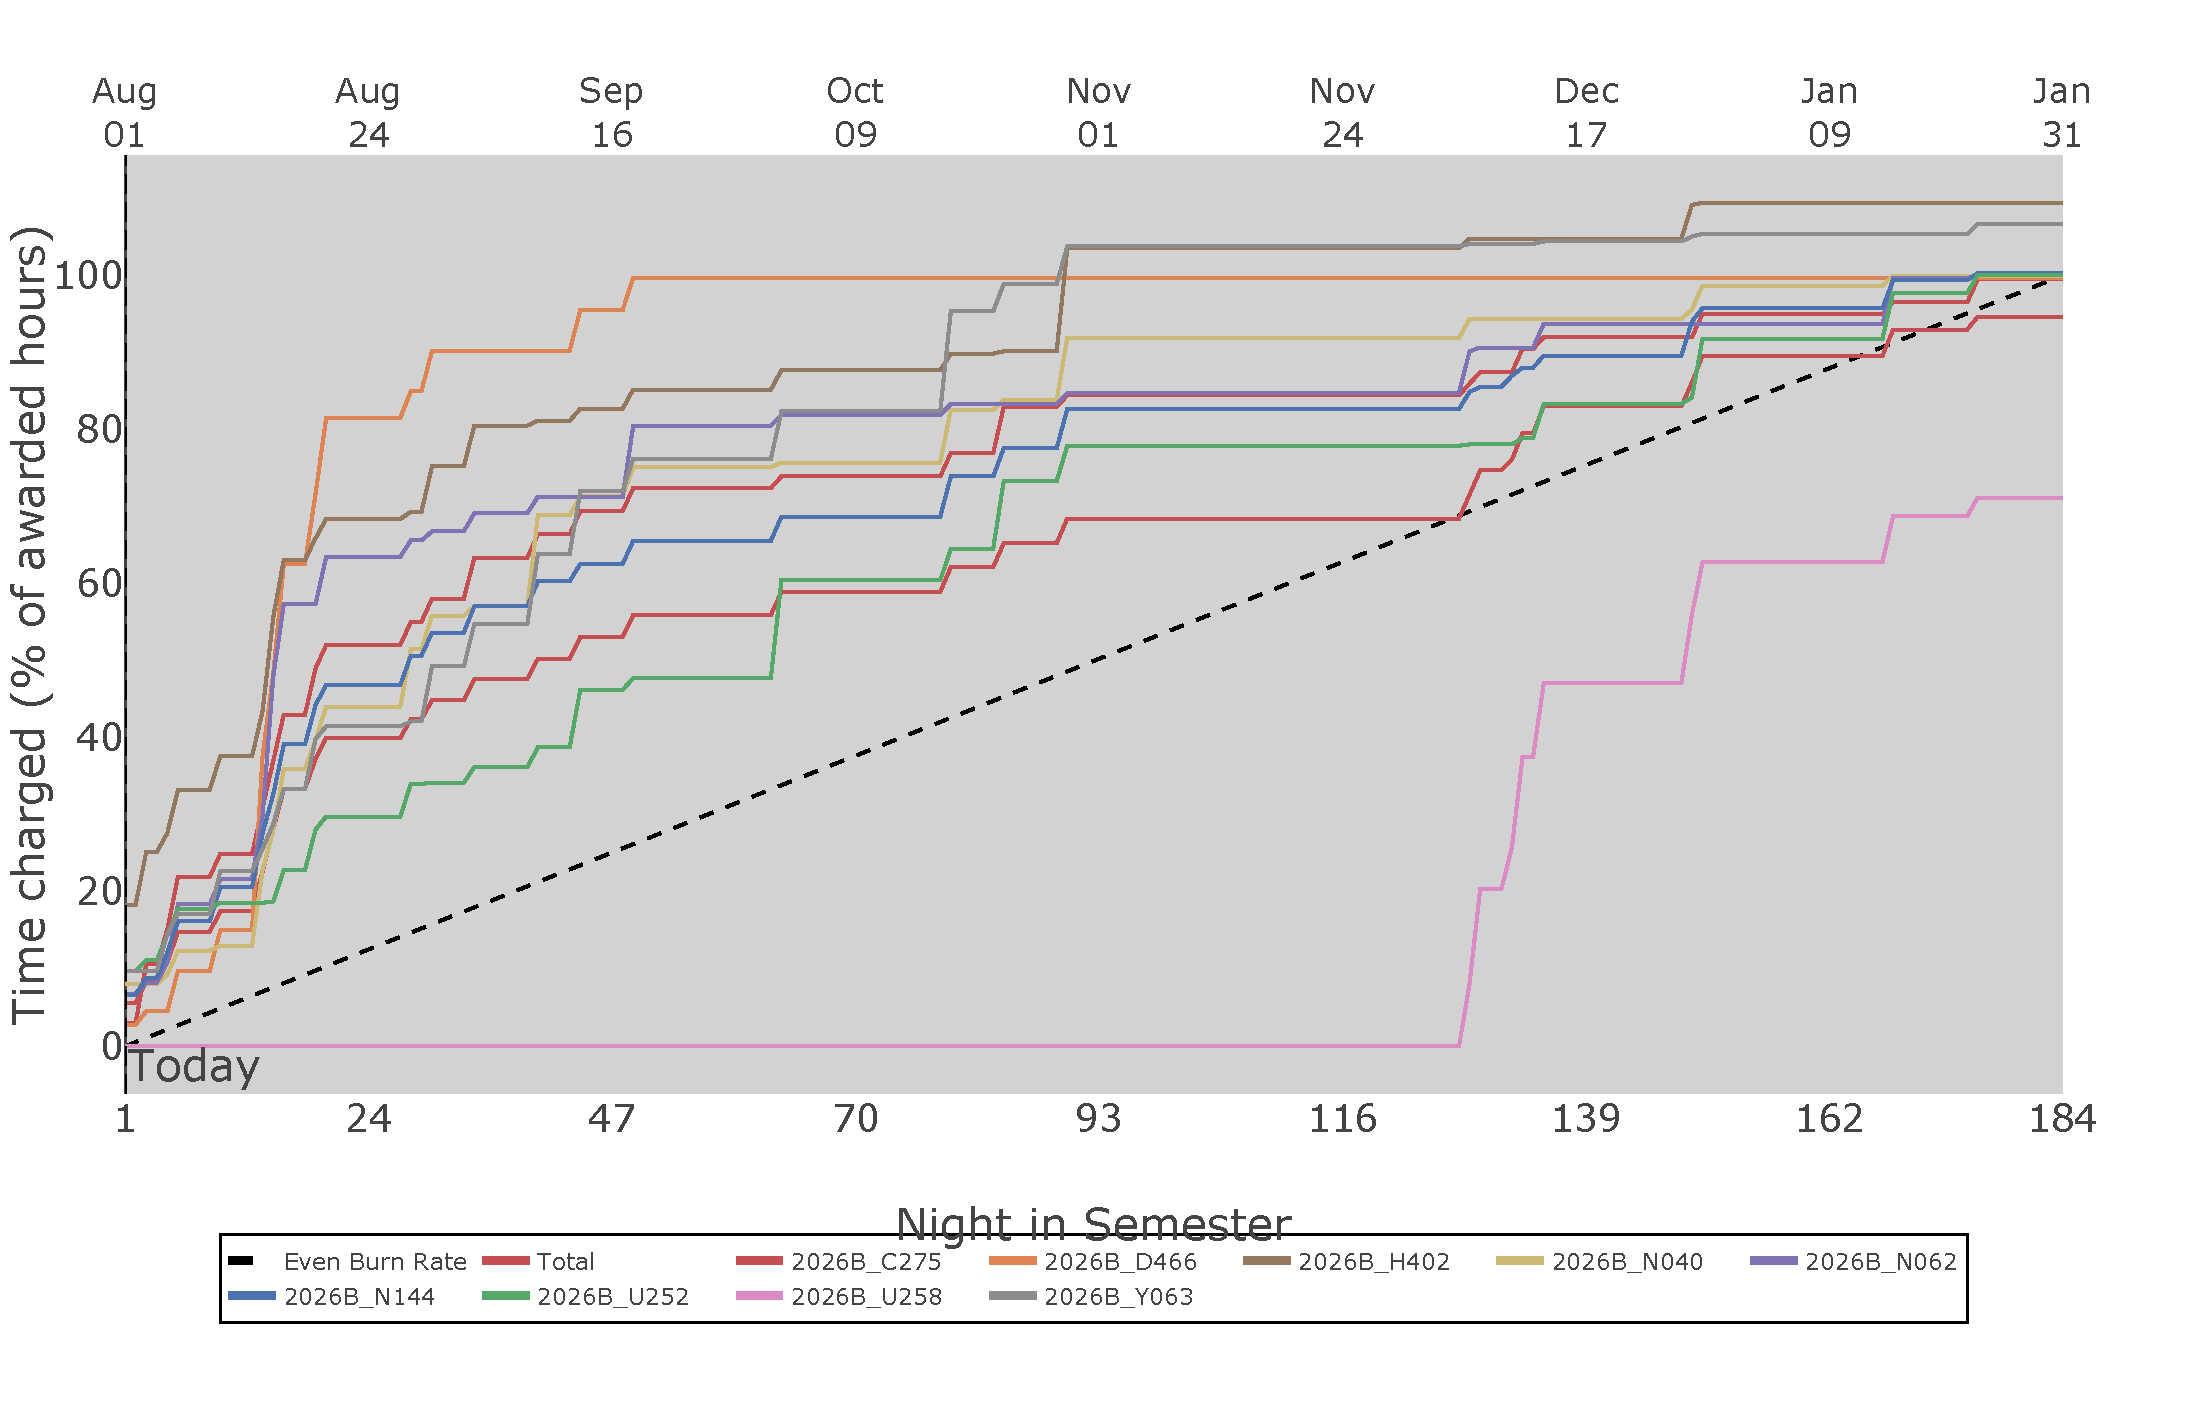
\includegraphics[width=0.88\textwidth]{plots/cof_hours.pdf}
  \caption{The plan constructed on the first night of the semester, viewed two
  ways. \emph{Upper:} each allocated night as a column of scheduling slots,
  colored by the program occupying it. Unallocated nights are blank, which is
  why the semester reads as isolated stripes. \emph{Lower:} cumulative time
  charged to each program as a percentage of its award, with the dashed line
  marking an even burn rate. U258 (pink) appears in neither panel until
  December and reaches only \param{base-u258-maff} of its award; the programs
  that finish above 100\% are absorbing the time it cannot use.
  \red{Caption to be finalized.}}
  \label{fig:cof}
\end{figure*}

Table~\ref{tab:programs} gives the corresponding per-program numbers. H402 and
Y063 end above their awards, which is possible only because stages 3 through 5
raise the fill ceiling to \param{pipeline-maxfill-late}. Under the ceiling of
unity that governs stages 1 and 2, that time would have gone unscheduled.

% GENERATED by tools/make_tables.py -- do not edit by hand.
\begin{deluxetable*}{lrrrrrr}
\tablecaption{Program-level statistics for the 2026B HIRES queue, as planned on the first night\label{tab:programs}}
\tablehead{
  \colhead{Program} & \colhead{$A_p$} & \colhead{Requested} &
  \colhead{Projected} & \colhead{\Fp} & \colhead{\maff} &
  \colhead{\fsf} \\
  \colhead{} & \colhead{(hr)} & \colhead{(hr)} & \colhead{(hr)} &
  \colhead{(\%)} & \colhead{(\%)} & \colhead{(\%)}
}
\startdata
C275 & 33.2 & 42.1 & 33.1 & 100 & 100 & 0 \\
C362\tablenotemark{b} & 0.0 & 0.0 & 0.0 & 0 & 0 & \nodata \\
D466 & 9.5 & 11.1 & 9.5 & 100 & 100 & 0 \\
E475\tablenotemark{a} & 600.0 & 0.0 & 0.0 & 0 & 0 & 0 \\
H402 & 10.7 & 14.4 & 11.7 & 109 & 100 & 0 \\
N040 & 5.4 & 7.0 & 5.4 & 100 & 100 & 0 \\
N062 & 14.1 & 18.9 & 14.1 & 100 & 100 & 0 \\
N144 & 25.5 & 30.7 & 25.6 & 100 & 100 & 0 \\
U252 & 19.7 & 22.6 & 19.7 & 100 & 100 & 0 \\
U258 & 36.1 & 36.5 & 25.7 & 71 & 71 & 0 \\
Y063 & 10.3 & 14.8 & 11.0 & 107 & 100 & 0
\enddata
\tablenotetext{a}{Filler backstop. Its award is nominal rather than allocated time and it is excluded from queue totals.}
\tablenotetext{b}{No requests submitted.}
\tablecomments{$A_p$ is the award, derived from the Keck blocks assigned to each program. \Fp is the projected fill, \maff the maximum feasible fill, and $\fsf = \maff - \Fp$ the fill shortfall of Equation~\ref{eq:fsf}. H402 and Y063 exceed 100\% because stages 3--5 raise the ceiling to \param{pipeline-maxfill-late}, letting them absorb time U258 cannot use (\S\ref{sec:balance:mismatch}).}
\end{deluxetable*}


\section{Balance Under Weather}
\label{sec:weather}

The queue described so far is never short of time: on a full allocation with no
losses, the only source of shortfall is the seasonal mismatch of
\S\ref{sec:balance:mismatch}. That makes it a poor test of the balance stage,
whose purpose is to decide who absorbs a shortage. Weather supplies the
shortage. This section reports a simulation of the semester as it would actually
be operated, night by night, with nights removed at random.

\subsection{Design}
\label{sec:weather:design}

We step through the \param{pair-nights} allocated nights of the semester in
order. On each night the semester plan is rebuilt from scratch, exactly as
\S\ref{sec:stages} describes and exactly as operations does it, using only the
information available that day. A Bernoulli draw with
$p = \param{pair-weather-p}\%$ then decides whether the night is wholly lost. If
it is clear, every visit the plan assigned to that night is appended to the
record of past observations and carried into the next night's replan; if it is
lost, nothing is banked. Losing a night is thus not modeled as a penalty term
but as the absence of data, which is what the scheduler actually sees.

Two properties of the design matter for interpreting the result.

\emph{The arms are paired.} The simulation is run twice on the same weather
realization: once with the full five-stage pipeline, and once with a four-stage
pipeline identical in every respect except that stage 2 is omitted. The
weighted-shortfall cap of Equation~\ref{eq:shortfall-cap} is applied in both, so the
control is held to the same tolerance on $Z$ as the balanced arm, and balance is
the only difference between them. The weather draw depends only on the seed and
the list of allocated nights, never on the arm, so both arms lose an identical
set of nights. Without such a control the experiment would be uninterpretable:
every program's fill falls when nights disappear, with or without balance.

\emph{Maximum feasible fill is recomputed nightly.} \maff is re-derived before
each replan, from the remaining allocation and the observations banked so far,
which is what \texttt{compute-max-fill} does in production. This has a
consequence worth stating plainly: as weather removes nights, \maff falls too,
so \fsf measures the gap to what a program could still achieve rather than to
what it was once promised. We therefore also record \fsf against \maff frozen at
its first-night value, which measures how far a program has fallen below what
looked achievable when the semester opened. The two readings answer different
questions and are reported separately.

\subsection{The shortage is real but the endpoint is not changed}
\label{sec:weather:result}

The realization reported here lost \param{pair-lost} of \param{pair-nights}
allocated nights, or \param{pair-lost-frac}\%. The shortfall stage proved
optimality on all \param{pair-shortfall-converged-bal} nights in both arms, with
a largest gap of \param{pair-shortfall-gap-max-bal}\%, so the non-convergence
that complicates \S\ref{sec:balance} is absent here.

Figure~\ref{fig:wxfsf} tracks the largest \fsf over all programs. Both arms sit
at zero through the first half of the semester, apart from one isolated night
(\param{pair-blip-date}), because until then enough time remains that no program
need give anything up. From \param{pair-split-date} they separate durably: the
unbalanced arm reaches \param{pair-fsf-peak-nobal} while balance holds the worst
program to \param{pair-fsf-peak-bal}. Averaged over the semester the worst \fsf
is \param{pair-fsf-mean-bal} with balance against \param{pair-fsf-mean-nobal}
without it.

The arms then converge, finishing at \param{pair-fsf-final-bal} and
\param{pair-fsf-final-nobal}. Measured against the frozen first-night \maff the
endpoints are \param{pair-frozen-final-bal} and
\param{pair-frozen-final-nobal}, and the two arms deliver the same total time to
within 0.1 hr (\param{pair-hours-bal} against
\param{pair-hours-nobal} of \param{pair-awarded} awarded). Balance changes who
is short during the semester without changing how much time the queue delivers
or, in this realization, where the worst-off program ends up.

\begin{figure}
  \centering
  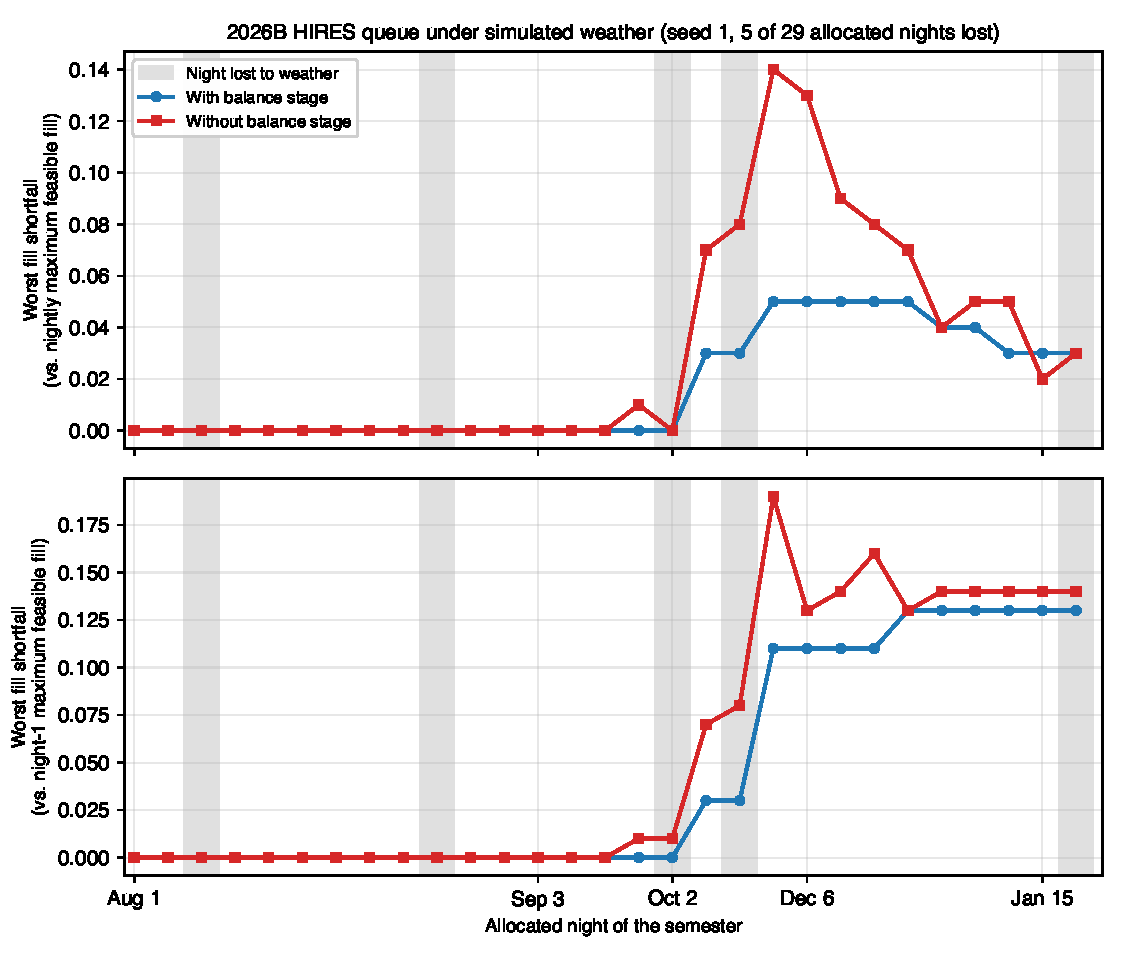
\includegraphics[width=\columnwidth]{plots/weather_fsf.pdf}
  \caption{Largest fill shortfall over all programs, with and without the
  balance stage, on a single weather realization. Shaded columns mark nights
  lost. \emph{Upper:} measured against \maff recomputed each night, the
  quantity stage 2 minimizes. \emph{Lower:} measured against \maff frozen at
  its first-night value. The horizontal axis is ordered by allocated night
  rather than by date, so the step between late October and early December
  spans five weeks in which the queue held no allocation.}
  \label{fig:wxfsf}
\end{figure}

\subsection{What balance actually redistributes}
\label{sec:weather:programs}

The envelope of Figure~\ref{fig:wxfsf} conceals the more informative result.
Broken out per program in Figure~\ref{fig:wxfsfprog}, the unbalanced arm turns
out to concentrate essentially all of the shortfall on two programs, C275 and
U258, while \param{pair-spared-nobal} of the \param{pair-nprograms} carry none
of it at all. Balance spreads the same shortage across the whole queue: the
programs that were spared entirely pick up a mean \fsf of
\param{pair-spared-mean-bal}, and the two that were carrying the shortage come
down.

Figure~\ref{fig:wxcomp} shows the same trade in units of completion. At the
worst of the weather, balance holds C275 at \param{pair-c275-dip-bal} of its
award where the unbalanced arm drops it to \param{pair-c275-dip-nobal}, and
U258 at \param{pair-u258-dip-bal} against \param{pair-u258-dip-nobal}. It pays
for this by pulling \param{pair-squeezed} programs that would otherwise sit at
or near their full award down to
\param{pair-squeezed-lo}--\param{pair-squeezed-hi}. The queue divides cleanly by
the sign of the change, \param{pair-protected} programs protected against
\param{pair-squeezed} squeezed, which is the signature of a max-min objective
and is not produced by any other stage of the pipeline.

Figure~\ref{fig:wxreal} shows realized rather than projected completion, and it
is included to make a negative point: the two arms track each other almost
exactly. What is actually banked is governed by which nights the weather took,
not by how the queue was balanced. Balance operates on the forecast, deciding
who is asked to give up time; it cannot create time.

\begin{figure*}
  \centering
  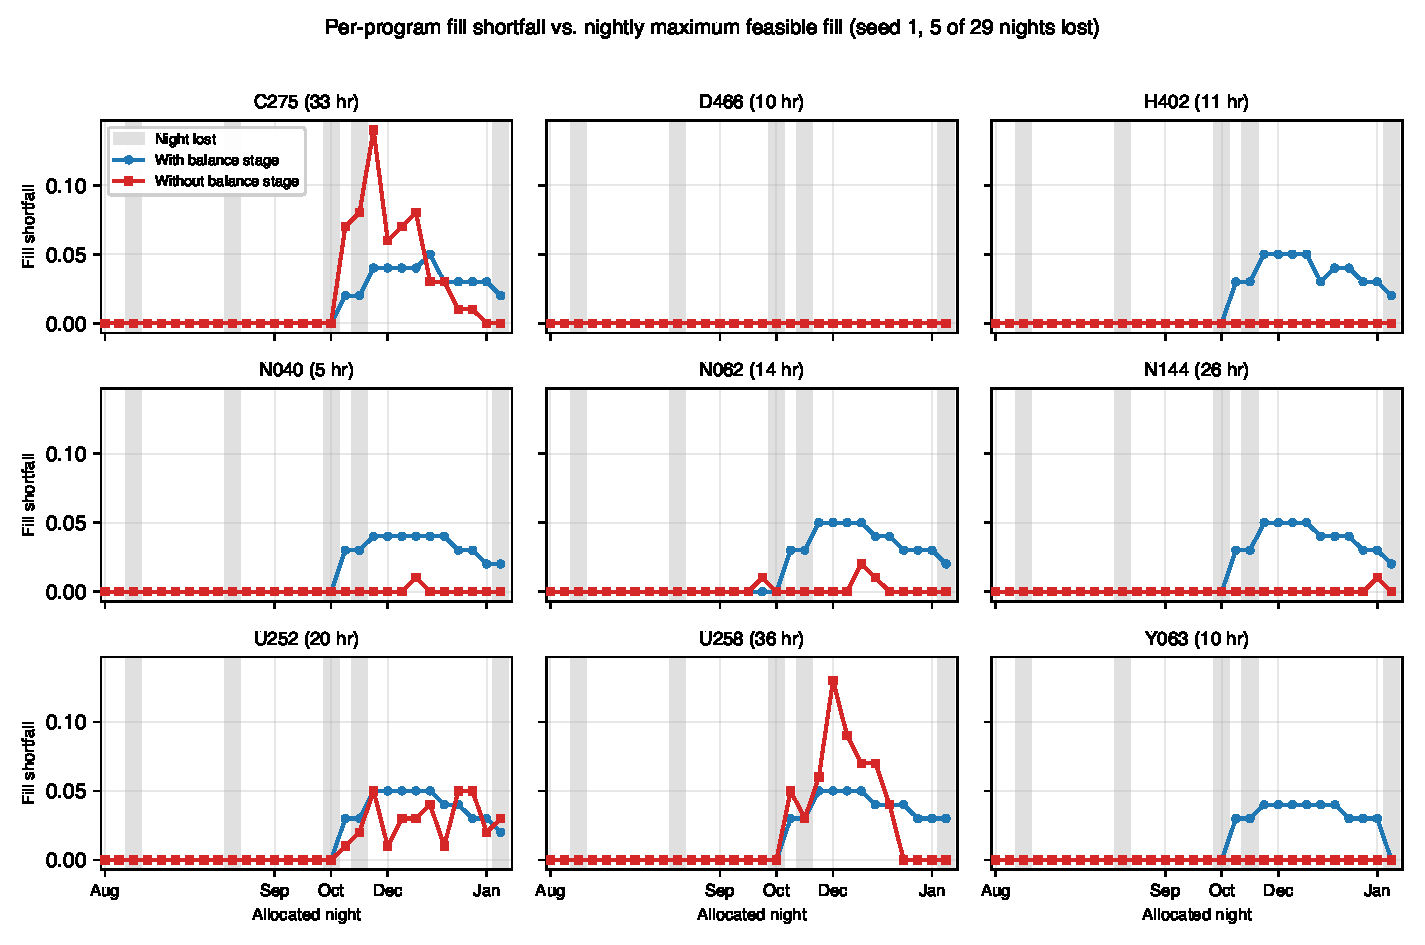
\includegraphics[width=\textwidth]{plots/weather_fsf_programs.pdf}
  \caption{Fill shortfall per program, measured against \maff recomputed
  nightly, for the same paired realization as Figure~\ref{fig:wxfsf}. Without
  balance the shortage falls almost entirely on C275 and U258 while
  \param{pair-spared-nobal} programs carry none; with balance it is spread
  across the queue at roughly 0.04--0.05. Shaded columns mark
  nights lost to weather.}
  \label{fig:wxfsfprog}
\end{figure*}

\begin{figure*}
  \centering
  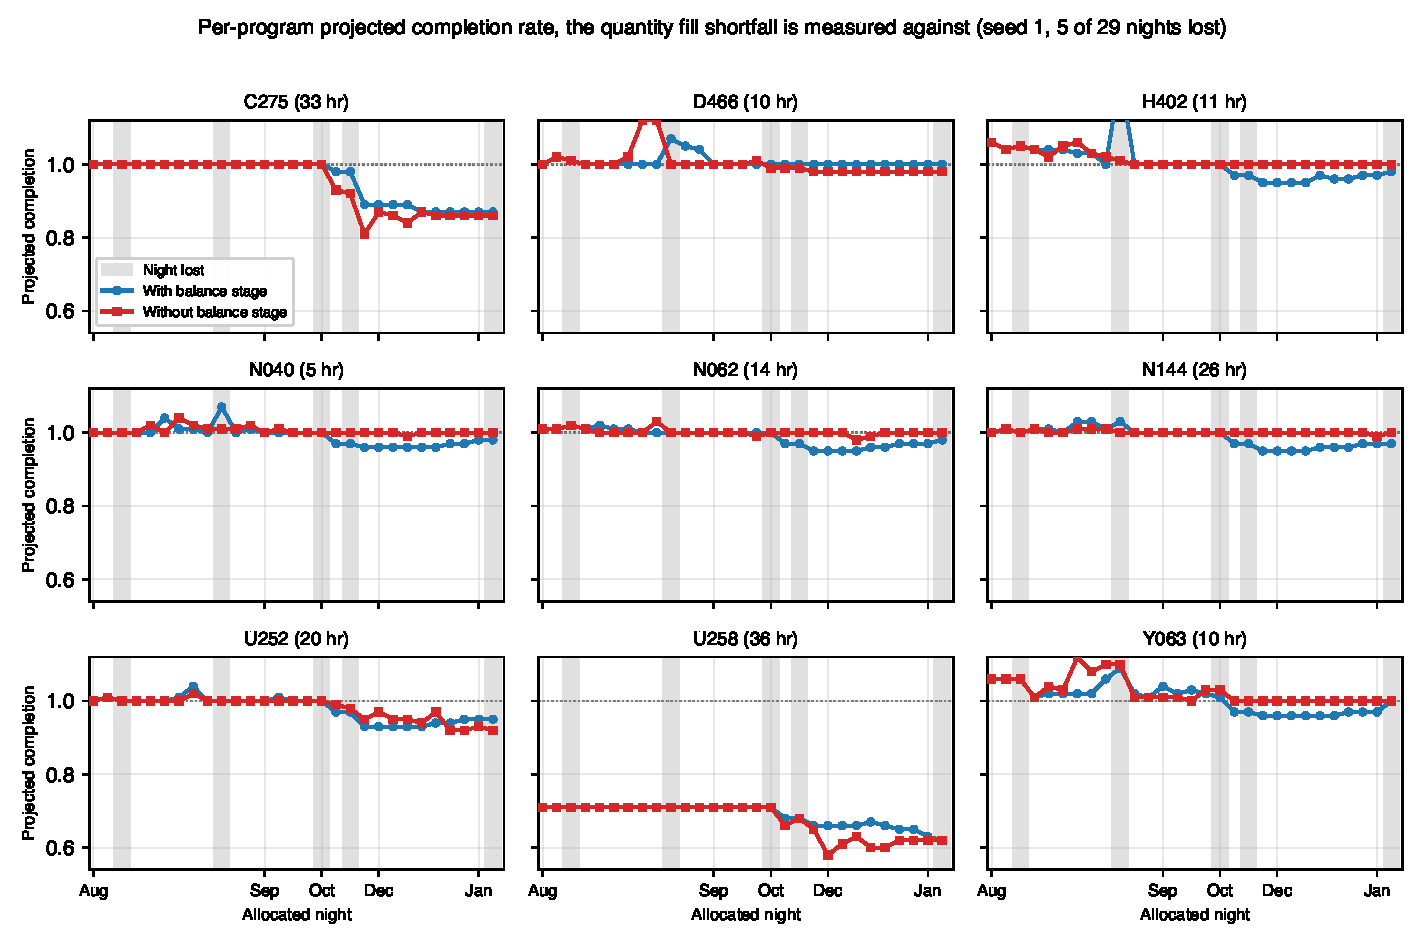
\includegraphics[width=\textwidth]{plots/weather_completion_programs.pdf}
  \caption{Projected completion rate per program, the quantity \fsf is measured
  against. Balance lifts the programs being squeezed and lowers those that
  would otherwise finish at their full award; the sign of the difference splits
  the queue in two.}
  \label{fig:wxcomp}
\end{figure*}

\begin{figure*}
  \centering
  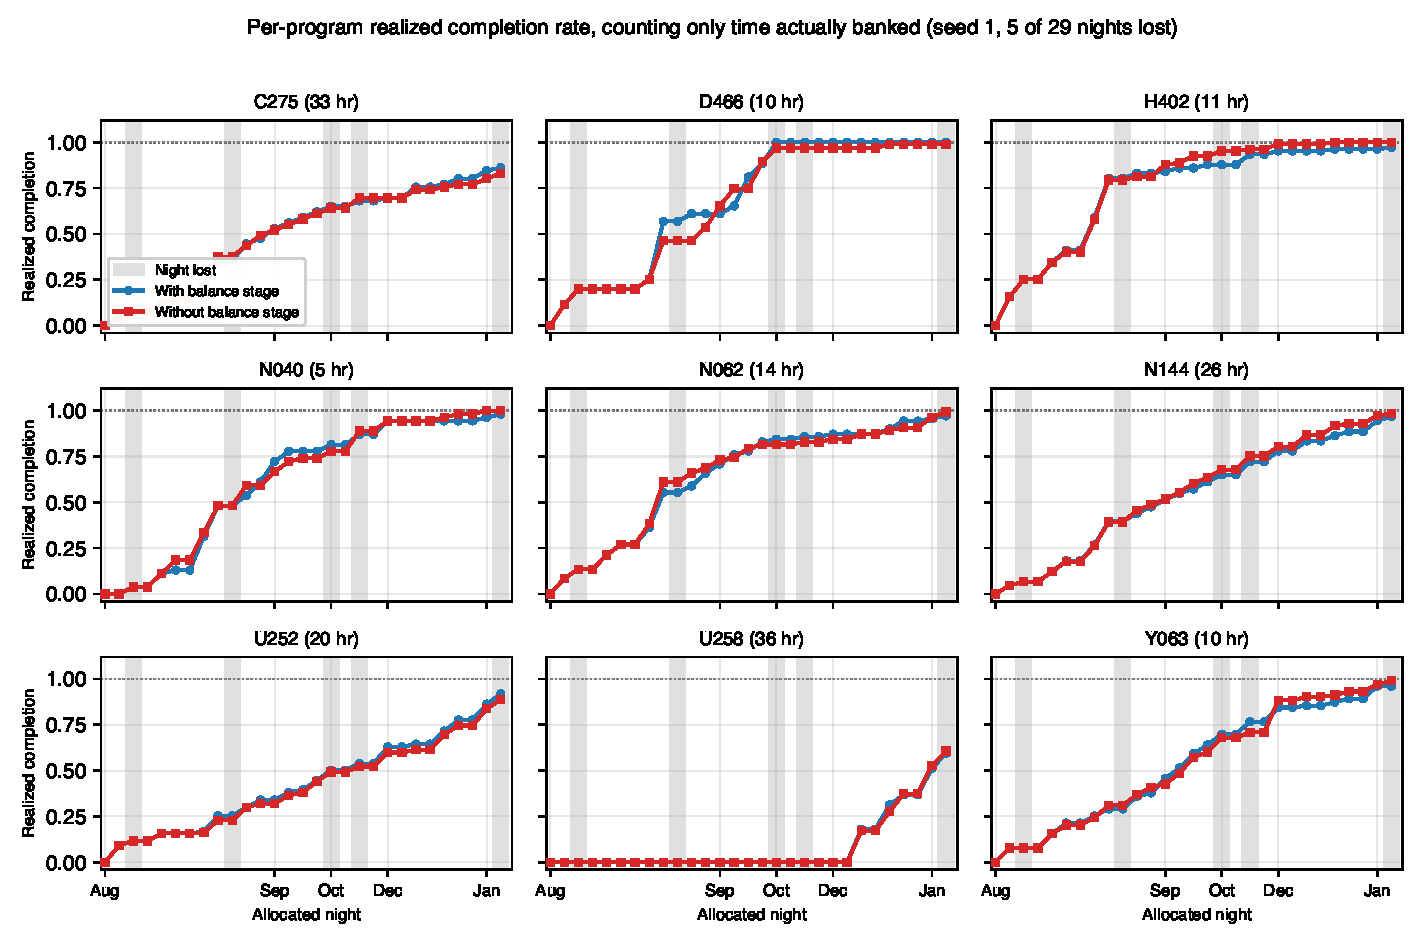
\includegraphics[width=\textwidth]{plots/weather_realized_programs.pdf}
  \caption{Realized completion rate per program, counting only time actually
  banked. The two arms are nearly identical: accumulation is set by which
  nights the weather took. U258 remains at zero until December regardless of
  arm. Curves end slightly below the projections of
  Figure~\ref{fig:wxcomp} because the last allocated night was itself lost.}
  \label{fig:wxreal}
\end{figure*}

\subsection{Limitations}
\label{sec:weather:limits}

This is one weather realization, and it lost \param{pair-lost-frac}\% of nights
against a \param{pair-weather-p}\% target, so it was a mild year in which the
queue had room to recover in January. A single draw cannot distinguish
``balance does not change the endpoint'' from ``this year was too easy to tell,''
and the convergence of the two arms in Figure~\ref{fig:wxfsf} should be read in
that light. The result that does not depend on the draw is the redistribution of
Figure~\ref{fig:wxfsfprog}, which is a property of the objective rather than of
the weather.

Two further caveats. The balance stage often failed to converge within its
\param{pair-balance-timelimit}\,s limit, leaving a gap above 1\% on
\param{pair-balance-loose} of the \param{pair-nights} nights and as much as
\param{pair-balance-gap-max}\% on one of them. This biases against balance, so
the advantage reported above is a lower bound on what the objective would
deliver if solved to optimality. And what counts as observed on a clear night is the semester plan's
assignment for that night rather than an executed night plan, so losses within
an otherwise clear night are not modeled. Details are recorded in
\texttt{notes/03-weather-paired-control.md}.

\section{Discussion}
\label{sec:discussion}

\red{To be drafted.}

\section{Conclusion}
\label{sec:conclusion}

\red{To be drafted.}

\section{Acknowledgments}

\red{To be drafted.}

\appendix

\section{Symbols used in this work}
\begin{table*}[h]
  \centering
  \caption{Dictionary of Variables}
  \label{variableDict}
  \begin{tabular}{cl}
    \hline
    Notation & \multicolumn{1}{c}{Description} \\
    \hline
    \hline

    \hfill \\
    \multicolumn{2}{l}{\textbf{Indices:}} \\
    $r$ & a request  \\
    $s$ & a slot  \\
    $d$ & a night \\
    $p$ & a program \\
    \hfill \\

    \multicolumn{2}{l}{\textbf{Grid Sizes:}} \\
    $N_r$ & Number of requests  \\
    $N_d$ & Number of nights in semester \\
    $N_s$ & Number of slots in a night  \\
    $N_p$ & Number of programs \\
    \hfill \\

    \multicolumn{2}{l}{\textbf{Sets:}} \\
    $\Rcal$ & Set of all requests \\
    $\Dcal$ & Set of all days \\
    $\Scal$ & Set of all slots \\
    $\Pcal$ & Set of all programs \\
    $\Rcal_p$ & $\{r \in \Rcal \mid \text{request $r$ belongs to program $p$} \}$ \\
    $\Tcal_{\rm alloc}$ & $\{(d,s) \in \Dcal \times \Scal \mid \text{slot $s$ of day $d$ is allocated to the queue} \}$ \\
    \hfill \\

    \multicolumn{2}{l}{\textbf{Observational Strategy:}} \\
    \isr{n}{intra, max, r} & Desired (maximum) number of visits per night for request $r$  \\
    \isr{n}{intra, min, r} & Accepted (minimum) number of visits per night for request $r$  \\
    \isr{\tau}{intra, r} & Minimum intra-night cadence for request $r$ \\
    \isr{n}{inter, r} & Maximum number of desired visits for request $r$  \\
    \isr{\tau}{inter, r} & Minimum inter-night cadence for request $r$ \\
    \isr{t}{visit, r} & The number of slots required to complete a visit for request $r$  \\
    $P_r$ & The number of past nights where request $r$ was observed \\
    \hfill \\

    \multicolumn{2}{l}{\textbf{Matrix Variables:}} \\
    $Y_{r,d,s}$ & Matrix of scheduled visits  \\
    $W_{r,d}$ & Matrix of on-sky visits, only for $r \in \Rcal_{\multivisit}$  \\
    $\Theta_r$ & Matrix of shortfall \\
    \hfill \\

    \multicolumn{2}{l}{\textbf{Program Balance:}} \\
    $A_p$ & Time awarded to program $p$, in slots \\
    \isr{A}{past,p} & Time already executed by program $p$, in slots \\
    $\Fp$ & Fill factor of program $p$: projected time as a fraction of $A_p$ \\
    $\minfill$ & Operator floor on $\Fp$ \\
    $\maxfill$ & Operator ceiling (throttle) on $\Fp$ \\
    $\maff$ & Maximum feasible fill: the $\Fp$ program $p$ attains with the telescope to itself \\
    $\fsf$ & Fill shortfall of program $p$, $\maff - \Fp$ \\
    $\fsfmax$ & The largest fill shortfall over all programs, minimized by the balance stage \\
    \hfill \\

    \multicolumn{2}{l}{\textbf{Staged Optimization:}} \\
    $Z$ & Time-weighted global shortfall, $\sum_r \Theta_r \isr{t}{visit,r}$ \\
    $\Zstar$ & The stage-1 optimum of $Z$ \\
    $\alpha$ & Slack multiplier; later stages require $Z \le \alpha \Zstar$ \\
    $\alpha_{\rm hold}$ & Fraction by which stage 3 relaxes the fill floor inherited from stage 2 \\
    $w_r$ & Intra-program priority weight of request $r$; smaller is higher priority \\
    $d_0$ & Index of the upcoming night \\
    $X^{(k)}$ & The value of quantity $X$ in the solution to stage $k$ \\
    \hfill \\

    \multicolumn{2}{l}{\textbf{Constants:}} \\
    $\tau_{\slot}$ & the time represented by one slot, in minutes \\

    \hline
  \end{tabular}
\end{table*}


\bibliography{bib.bib}

\end{document}
